\documentclass{standalone}
\usepackage{tikz}
\usetikzlibrary{patterns, positioning}


\begin{document}
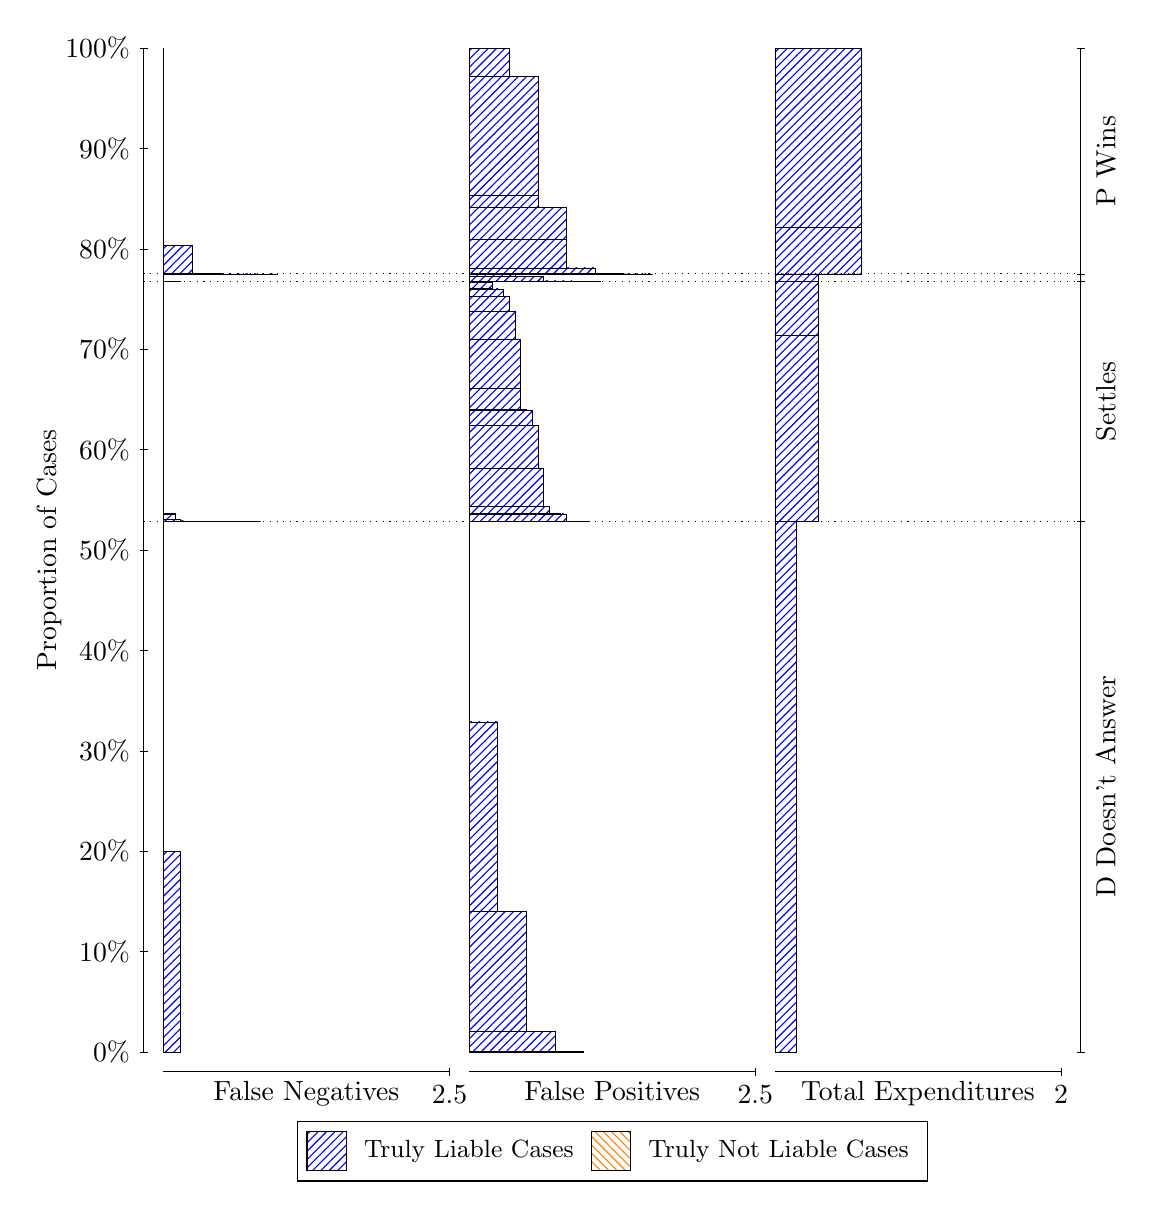
\begin{tikzpicture}
\draw[black, very thin] (1.5,1.75) -- (1.5,14.5);
\node[rotate=90, text=black, anchor=center] at (0.3, 8.125) {Proportion of Cases};
\draw[black, very thin] (1.45,1.75) -- (1.55,1.75);
\node[text=black, anchor=east] at (1.45, 1.75) {0\%};
\draw[black, very thin] (1.45,3.025) -- (1.55,3.025);
\node[text=black, anchor=east] at (1.45, 3.025) {10\%};
\draw[black, very thin] (1.45,4.3) -- (1.55,4.3);
\node[text=black, anchor=east] at (1.45, 4.3) {20\%};
\draw[black, very thin] (1.45,5.575) -- (1.55,5.575);
\node[text=black, anchor=east] at (1.45, 5.575) {30\%};
\draw[black, very thin] (1.45,6.85) -- (1.55,6.85);
\node[text=black, anchor=east] at (1.45, 6.85) {40\%};
\draw[black, very thin] (1.45,8.125) -- (1.55,8.125);
\node[text=black, anchor=east] at (1.45, 8.125) {50\%};
\draw[black, very thin] (1.45,9.4) -- (1.55,9.4);
\node[text=black, anchor=east] at (1.45, 9.4) {60\%};
\draw[black, very thin] (1.45,10.675) -- (1.55,10.675);
\node[text=black, anchor=east] at (1.45, 10.675) {70\%};
\draw[black, very thin] (1.45,11.95) -- (1.55,11.95);
\node[text=black, anchor=east] at (1.45, 11.95) {80\%};
\draw[black, very thin] (1.45,13.225) -- (1.55,13.225);
\node[text=black, anchor=east] at (1.45, 13.225) {90\%};
\draw[black, very thin] (1.45,14.5) -- (1.55,14.5);
\node[text=black, anchor=east] at (1.45, 14.5) {100\%};

\draw[black, very thin] (13.4,1.75) -- (13.4,14.5);
\draw[black, very thin] (13.35,1.75) -- (13.45,1.75);
\node[anchor=west] at (13.35, 1.75) {};
\draw[black, very thin] (13.35,8.4895) -- (13.45,8.4895);
\node[anchor=west] at (13.35, 8.4895) {};
\draw[black, very thin] (13.35,11.54) -- (13.45,11.54);
\node[anchor=west] at (13.35, 11.54) {};
\draw[black, very thin] (13.35,11.633) -- (13.45,11.633);
\node[anchor=west] at (13.35, 11.633) {};
\draw[black, very thin] (13.35,14.5) -- (13.45,14.5);
\node[anchor=west] at (13.35, 14.5) {};

\draw[black, very thin, pattern color=blue, pattern=north east lines] (1.75,1.75) rectangle (1.968,4.2985);
\draw[black, very thin, pattern color=orange, pattern=north west lines] (1.75,4.2985) rectangle (1.75,4.2985);
\draw[black, very thin, pattern color=blue, pattern=north east lines] (1.75,4.2985) rectangle (1.75,8.4895);
\draw[black, very thin, pattern color=blue, pattern=north east lines] (1.75,8.4895) rectangle (2.9853,8.4895);
\draw[black, very thin, pattern color=blue, pattern=north east lines] (1.75,8.4895) rectangle (2.6947,8.4895);
\draw[black, very thin, pattern color=blue, pattern=north east lines] (1.75,8.4895) rectangle (2.622,8.4895);
\draw[black, very thin, pattern color=blue, pattern=north east lines] (1.75,8.4895) rectangle (2.5493,8.4895);
\draw[black, very thin, pattern color=blue, pattern=north east lines] (1.75,8.4895) rectangle (2.404,8.4895);
\draw[black, very thin, pattern color=blue, pattern=north east lines] (1.75,8.4895) rectangle (2.3313,8.4895);
\draw[black, very thin, pattern color=blue, pattern=north east lines] (1.75,8.4895) rectangle (2.2587,8.4896);
\draw[black, very thin, pattern color=blue, pattern=north east lines] (1.75,8.4896) rectangle (2.186,8.4896);
\draw[black, very thin, pattern color=blue, pattern=north east lines] (1.75,8.4896) rectangle (2.1133,8.4907);
\draw[black, very thin, pattern color=blue, pattern=north east lines] (1.75,8.4907) rectangle (2.0407,8.495);
\draw[black, very thin, pattern color=blue, pattern=north east lines] (1.75,8.495) rectangle (1.968,8.5101);
\draw[black, very thin, pattern color=blue, pattern=north east lines] (1.75,8.5101) rectangle (1.8953,8.5769);
\draw[black, very thin, pattern color=blue, pattern=north east lines] (1.75,8.5769) rectangle (1.8953,8.5877);
\draw[black, very thin, pattern color=blue, pattern=north east lines] (1.75,8.5877) rectangle (1.8227,8.588);
\draw[black, very thin, pattern color=orange, pattern=north west lines] (1.75,8.588) rectangle (1.75,8.588);
\draw[black, very thin, pattern color=blue, pattern=north east lines] (1.75,8.588) rectangle (1.75,11.54);
\draw[black, very thin, pattern color=blue, pattern=north east lines] (1.75,11.54) rectangle (1.968,11.541);
\draw[black, very thin, pattern color=orange, pattern=north west lines] (1.75,11.541) rectangle (1.75,11.541);
\draw[black, very thin, pattern color=blue, pattern=north east lines] (1.75,11.541) rectangle (1.75,11.633);
\draw[black, very thin, pattern color=blue, pattern=north east lines] (1.75,11.633) rectangle (3.2033,11.633);
\draw[black, very thin, pattern color=blue, pattern=north east lines] (1.75,11.633) rectangle (2.84,11.633);
\draw[black, very thin, pattern color=blue, pattern=north east lines] (1.75,11.633) rectangle (2.4767,11.639);
\draw[black, very thin, pattern color=blue, pattern=north east lines] (1.75,11.639) rectangle (2.1133,11.997);
\draw[black, very thin, pattern color=orange, pattern=north west lines] (1.75,11.997) rectangle (1.75,11.997);
\draw[black, very thin, pattern color=blue, pattern=north east lines] (1.75,11.997) rectangle (1.75,14.5);
\draw[black, very thin, pattern color=orange, pattern=north west lines] (5.6333,1.75) rectangle (7.0867,1.75);
\draw[black, very thin, pattern color=blue, pattern=north east lines] (5.6333,1.75) rectangle (7.0867,1.7526);
\draw[black, very thin, pattern color=blue, pattern=north east lines] (5.6333,1.7526) rectangle (6.7233,2.0143);
\draw[black, very thin, pattern color=blue, pattern=north east lines] (5.6333,2.0143) rectangle (6.36,3.538);
\draw[black, very thin, pattern color=blue, pattern=north east lines] (5.6333,3.538) rectangle (5.9967,5.9411);
\draw[black, very thin, pattern color=blue, pattern=north east lines] (5.6333,5.9411) rectangle (5.6333,8.4895);
\draw[black, very thin, pattern color=orange, pattern=north west lines] (5.6333,8.4895) rectangle (7.1593,8.4895);
\draw[black, very thin, pattern color=blue, pattern=north east lines] (5.6333,8.4895) rectangle (7.1593,8.4895);
\draw[black, very thin, pattern color=orange, pattern=north west lines] (5.6333,8.4895) rectangle (7.014,8.4895);
\draw[black, very thin, pattern color=blue, pattern=north east lines] (5.6333,8.4895) rectangle (7.014,8.4901);
\draw[black, very thin, pattern color=orange, pattern=north west lines] (5.6333,8.4901) rectangle (6.8687,8.4901);
\draw[black, very thin, pattern color=blue, pattern=north east lines] (5.6333,8.4901) rectangle (6.8687,8.5848);
\draw[black, very thin, pattern color=blue, pattern=north east lines] (5.6333,8.5848) rectangle (6.796,8.591);
\draw[black, very thin, pattern color=orange, pattern=north west lines] (5.6333,8.591) rectangle (6.7233,8.591);
\draw[black, very thin, pattern color=blue, pattern=north east lines] (5.6333,8.591) rectangle (6.7233,8.5914);
\draw[black, very thin, pattern color=blue, pattern=north east lines] (5.6333,8.5914) rectangle (6.6507,8.6764);
\draw[black, very thin, pattern color=orange, pattern=north west lines] (5.6333,8.6764) rectangle (6.578,8.6764);
\draw[black, very thin, pattern color=blue, pattern=north east lines] (5.6333,8.6764) rectangle (6.578,9.1648);
\draw[black, very thin, pattern color=blue, pattern=north east lines] (5.6333,9.1648) rectangle (6.5053,9.7113);
\draw[black, very thin, pattern color=blue, pattern=north east lines] (5.6333,9.7113) rectangle (6.4327,9.8987);
\draw[black, very thin, pattern color=blue, pattern=north east lines] (5.6333,9.8987) rectangle (6.36,9.9064);
\draw[black, very thin, pattern color=blue, pattern=north east lines] (5.6333,9.9064) rectangle (6.2873,10.174);
\draw[black, very thin, pattern color=orange, pattern=north west lines] (5.6333,10.174) rectangle (6.2873,10.174);
\draw[black, very thin, pattern color=blue, pattern=north east lines] (5.6333,10.174) rectangle (6.2873,10.798);
\draw[black, very thin, pattern color=blue, pattern=north east lines] (5.6333,10.798) rectangle (6.2147,11.152);
\draw[black, very thin, pattern color=blue, pattern=north east lines] (5.6333,11.152) rectangle (6.142,11.346);
\draw[black, very thin, pattern color=blue, pattern=north east lines] (5.6333,11.346) rectangle (6.0693,11.442);
\draw[black, very thin, pattern color=blue, pattern=north east lines] (5.6333,11.442) rectangle (5.9967,11.442);
\draw[black, very thin, pattern color=blue, pattern=north east lines] (5.6333,11.442) rectangle (5.924,11.453);
\draw[black, very thin, pattern color=blue, pattern=north east lines] (5.6333,11.453) rectangle (5.924,11.52);
\draw[black, very thin, pattern color=blue, pattern=north east lines] (5.6333,11.52) rectangle (5.8513,11.535);
\draw[black, very thin, pattern color=blue, pattern=north east lines] (5.6333,11.535) rectangle (5.7787,11.539);
\draw[black, very thin, pattern color=blue, pattern=north east lines] (5.6333,11.539) rectangle (5.706,11.54);
\draw[black, very thin, pattern color=blue, pattern=north east lines] (5.6333,11.54) rectangle (5.6333,11.54);
\draw[black, very thin, pattern color=orange, pattern=north west lines] (5.6333,11.54) rectangle (7.3047,11.54);
\draw[black, very thin, pattern color=blue, pattern=north east lines] (5.6333,11.54) rectangle (7.3047,11.54);
\draw[black, very thin, pattern color=blue, pattern=north east lines] (5.6333,11.54) rectangle (6.9413,11.542);
\draw[black, very thin, pattern color=blue, pattern=north east lines] (5.6333,11.542) rectangle (6.578,11.6);
\draw[black, very thin, pattern color=blue, pattern=north east lines] (5.6333,11.6) rectangle (6.2147,11.632);
\draw[black, very thin, pattern color=blue, pattern=north east lines] (5.6333,11.632) rectangle (5.8513,11.633);
\draw[black, very thin, pattern color=orange, pattern=north west lines] (5.6333,11.633) rectangle (7.9587,11.633);
\draw[black, very thin, pattern color=blue, pattern=north east lines] (5.6333,11.633) rectangle (7.9587,11.633);
\draw[black, very thin, pattern color=orange, pattern=north west lines] (5.6333,11.633) rectangle (7.5953,11.633);
\draw[black, very thin, pattern color=blue, pattern=north east lines] (5.6333,11.633) rectangle (7.5953,11.634);
\draw[black, very thin, pattern color=orange, pattern=north west lines] (5.6333,11.634) rectangle (7.232,11.634);
\draw[black, very thin, pattern color=blue, pattern=north east lines] (5.6333,11.634) rectangle (7.232,11.709);
\draw[black, very thin, pattern color=blue, pattern=north east lines] (5.6333,11.709) rectangle (6.8687,12.066);
\draw[black, very thin, pattern color=orange, pattern=north west lines] (5.6333,12.066) rectangle (6.8687,12.066);
\draw[black, very thin, pattern color=blue, pattern=north east lines] (5.6333,12.066) rectangle (6.8687,12.478);
\draw[black, very thin, pattern color=blue, pattern=north east lines] (5.6333,12.478) rectangle (6.5053,12.631);
\draw[black, very thin, pattern color=orange, pattern=north west lines] (5.6333,12.631) rectangle (6.5053,12.631);
\draw[black, very thin, pattern color=blue, pattern=north east lines] (5.6333,12.631) rectangle (6.5053,14.135);
\draw[black, very thin, pattern color=blue, pattern=north east lines] (5.6333,14.135) rectangle (6.142,14.136);
\draw[black, very thin, pattern color=blue, pattern=north east lines] (5.6333,14.136) rectangle (6.142,14.493);
\draw[black, very thin, pattern color=blue, pattern=north east lines] (5.6333,14.493) rectangle (5.7787,14.493);
\draw[black, very thin, pattern color=blue, pattern=north east lines] (5.6333,14.493) rectangle (5.7787,14.5);
\draw[black, very thin, pattern color=blue, pattern=north east lines] (5.6333,14.5) rectangle (5.6333,14.5);
\draw[black, very thin, pattern color=orange, pattern=north west lines] (9.5167,1.75) rectangle (9.7892,1.75);
\draw[black, very thin, pattern color=blue, pattern=north east lines] (9.5167,1.75) rectangle (9.7892,8.4895);
\draw[black, very thin, pattern color=orange, pattern=north west lines] (9.5167,8.4895) rectangle (10.062,8.4895);
\draw[black, very thin, pattern color=blue, pattern=north east lines] (9.5167,8.4895) rectangle (10.062,10.849);
\draw[black, very thin, pattern color=orange, pattern=north west lines] (9.5167,10.849) rectangle (10.062,10.849);
\draw[black, very thin, pattern color=blue, pattern=north east lines] (9.5167,10.849) rectangle (10.062,11.54);
\draw[black, very thin, pattern color=orange, pattern=north west lines] (9.5167,11.54) rectangle (10.062,11.54);
\draw[black, very thin, pattern color=blue, pattern=north east lines] (9.5167,11.54) rectangle (10.062,11.633);
\draw[black, very thin, pattern color=orange, pattern=north west lines] (9.5167,11.633) rectangle (10.607,11.633);
\draw[black, very thin, pattern color=blue, pattern=north east lines] (9.5167,11.633) rectangle (10.607,12.22);
\draw[black, very thin, pattern color=orange, pattern=north west lines] (9.5167,12.22) rectangle (10.607,12.22);
\draw[black, very thin, pattern color=blue, pattern=north east lines] (9.5167,12.22) rectangle (10.607,14.5);
\draw[black, dotted] (1.5,8.4895) -- (13.4,8.4895);
\draw[black, dotted] (1.5,11.54) -- (13.4,11.54);
\draw[black, dotted] (1.5,11.633) -- (13.4,11.633);
\draw[black, very thin] (1.75,1.5) -- (5.3833,1.5);
\node[text=black, anchor=north] at (3.5667, 1.5) {False Negatives};
\draw[black, very thin] (5.3833,1.45) -- (5.3833,1.55);
\node[text=black, anchor=north] at (5.3833, 1.45) {2.5};

\draw[black, very thin] (5.6333,1.5) -- (9.2667,1.5);
\node[text=black, anchor=north] at (7.45, 1.5) {False Positives};
\draw[black, very thin] (9.2667,1.45) -- (9.2667,1.55);
\node[text=black, anchor=north] at (9.2667, 1.45) {2.5};

\draw[black, very thin] (9.5167,1.5) -- (13.15,1.5);
\node[text=black, anchor=north] at (11.333, 1.5) {Total Expenditures};
\draw[black, very thin] (13.15,1.45) -- (13.15,1.55);
\node[text=black, anchor=north] at (13.15, 1.45) {2};

\node[text=black, centered, rotate=90] at (13.72, 5.1198) {D Doesn't Answer};
\node[text=black, centered, rotate=90] at (13.72, 10.015) {Settles};

\node[text=black, centered, rotate=90] at (13.72, 13.066) {P Wins};

\draw (7.449999999999999,1.5) node[draw=none] (baseCoordinate) {};
\begin{scope}[align=center]
        \matrix[scale=0.5, draw=black, below=0.5cm of baseCoordinate, nodes={draw}, column sep=0.1cm]{
            \node[rectangle, draw, minimum width=0.5cm, minimum height=0.5cm, pattern color=blue, pattern=north east lines] {}; &
            \node[draw=none, font=\small, text=black] (B) {Truly Liable Cases}; &
            \node[rectangle, draw, minimum width=0.5cm, minimum height=0.5cm, pattern color=orange, pattern=north west lines] {}; &
            \node[draw=none, font=\small, text=black] (B) {Truly Not Liable Cases}; \\
            };
\end{scope}

\end{tikzpicture}
\end{document}